\section{Моделирование 
  физических процессов,
  протекающих в проектируемом
  радиоэлектронном средстве}

% В данном разделе будет приведены данные о моделировании устройства в
% следующих программах:
% \begin{itemize}
% \item Ansys,
  
% \item COMSOL Multiphysics,
% \item Solidworks Simulation,
  
% \item Solidworks Flow Simulation.
% \end{itemize}

% Будет приведена инфомарция касательно результатов моделирования данных
% программах.

\subsection{Обоснование выбора пакетов 
  прикладного программного обеспечения 
  ANSYS, COMSOL Multiphysics, SolidWorks Simulation
 для моделирования физических процессов, протекающих в РЭС}

Популярность таких программ как COMSOL Multiphysics и
ANSYS в кругах инженеров позволяет рассчитывать на наличие
большого количетства обучающих материалов по ним, в том числе
созданных не только самой компанией осуществляющей разработку
программы.

Кроме того обе программы сами по себе обладают огромным набором
возможностей для проведения симуляции и зачастую имеют некоторый
аналог интерфейса трёхмерных параметрических САПР типа
SOLIDWORKS, который позволяет интерактивно взаимодествовать с
геометрией модели, материалом и сеткой модели.

Также особенно хочется отметить доступность и качество документации
доступной на официальном сайте COMSOL.

Совокупноcть вышеописанных качеств делает эти программы достойным
выбором для проведения исследования.

\subsection{Компоененты математического обеспечения пакетов
  ANSYS, COMSOL Multiphysics, SolidWorks Simulation
  для автоматизированного анализа физических процессов протекающих в РЭС}

\subsection{Технология построения трехмерных моделей исследуемого
  устройства в средах ANSYS, COMSOL Multiphysics, SolidWorks Simulation}

\subsection{Технология моделирования механических процессов,
протекающих в электронном модуле и устройстве в целом с
использованием ANSYS, COMSOL Multiphysics, SolidWorks Simulation}

В моделирование механических процессов вклачает частотный анализ
печатной платы. Эксперимент проводится в среде SolidWorks Simulation.

\begin{figure}[H]
  \centering
  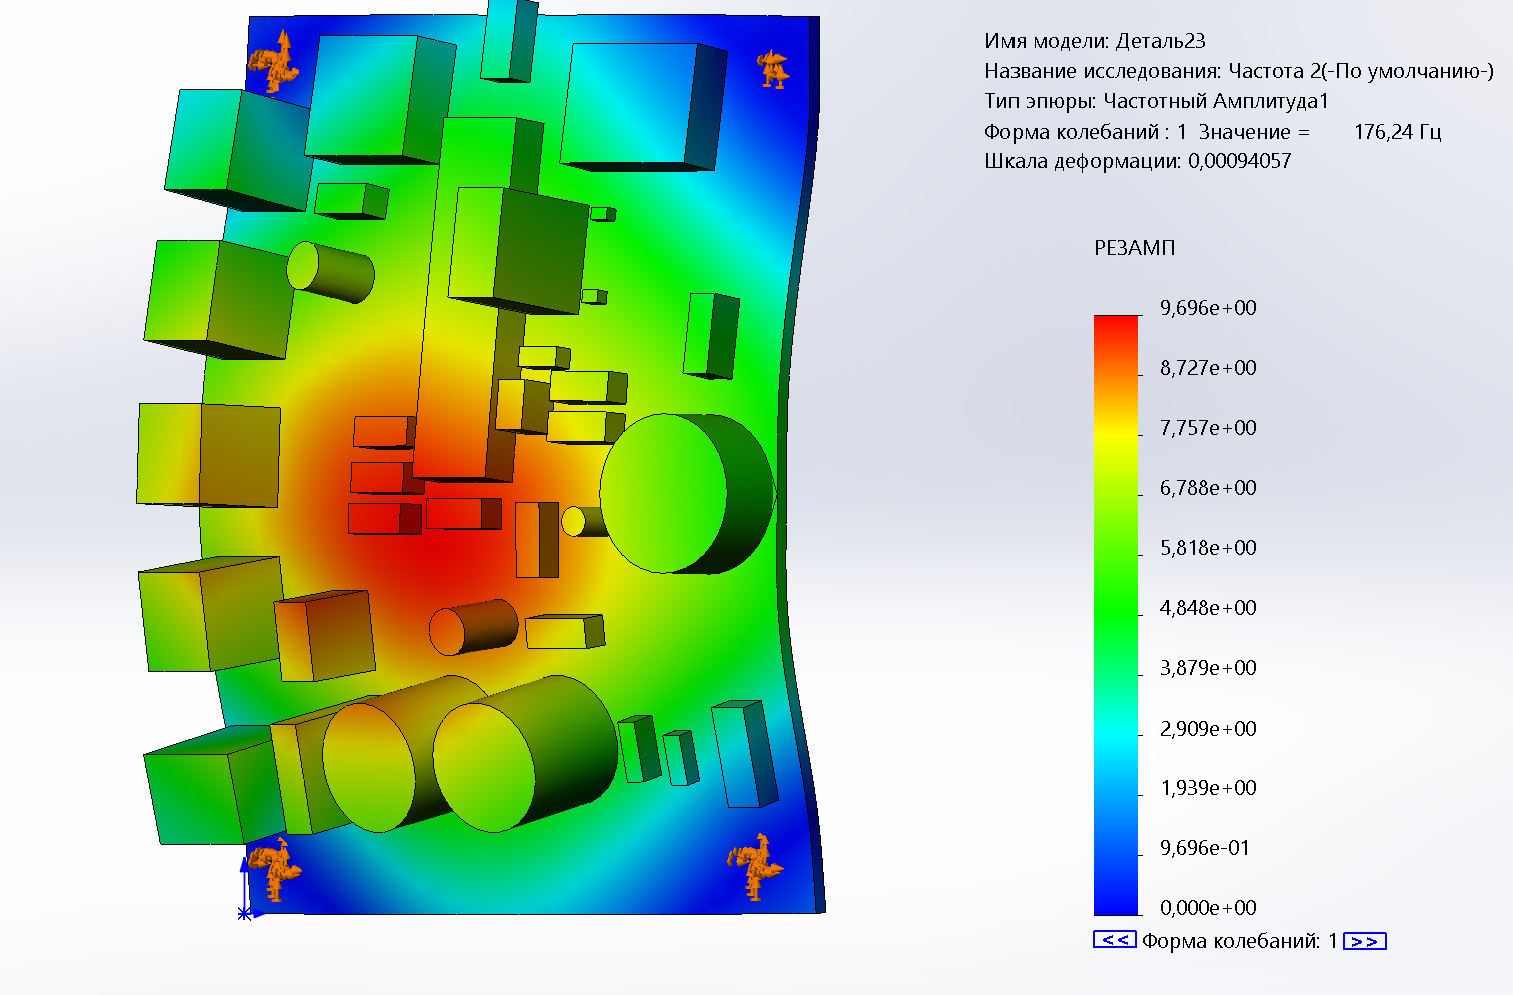
\includegraphics[scale=0.5]{solid.modeling/Amplitude-1-1.png}
  \caption{Результат эксперемента в SolidWorks Simulation (вариант 1)}
\end{figure}

\begin{figure}[H]
  \centering
  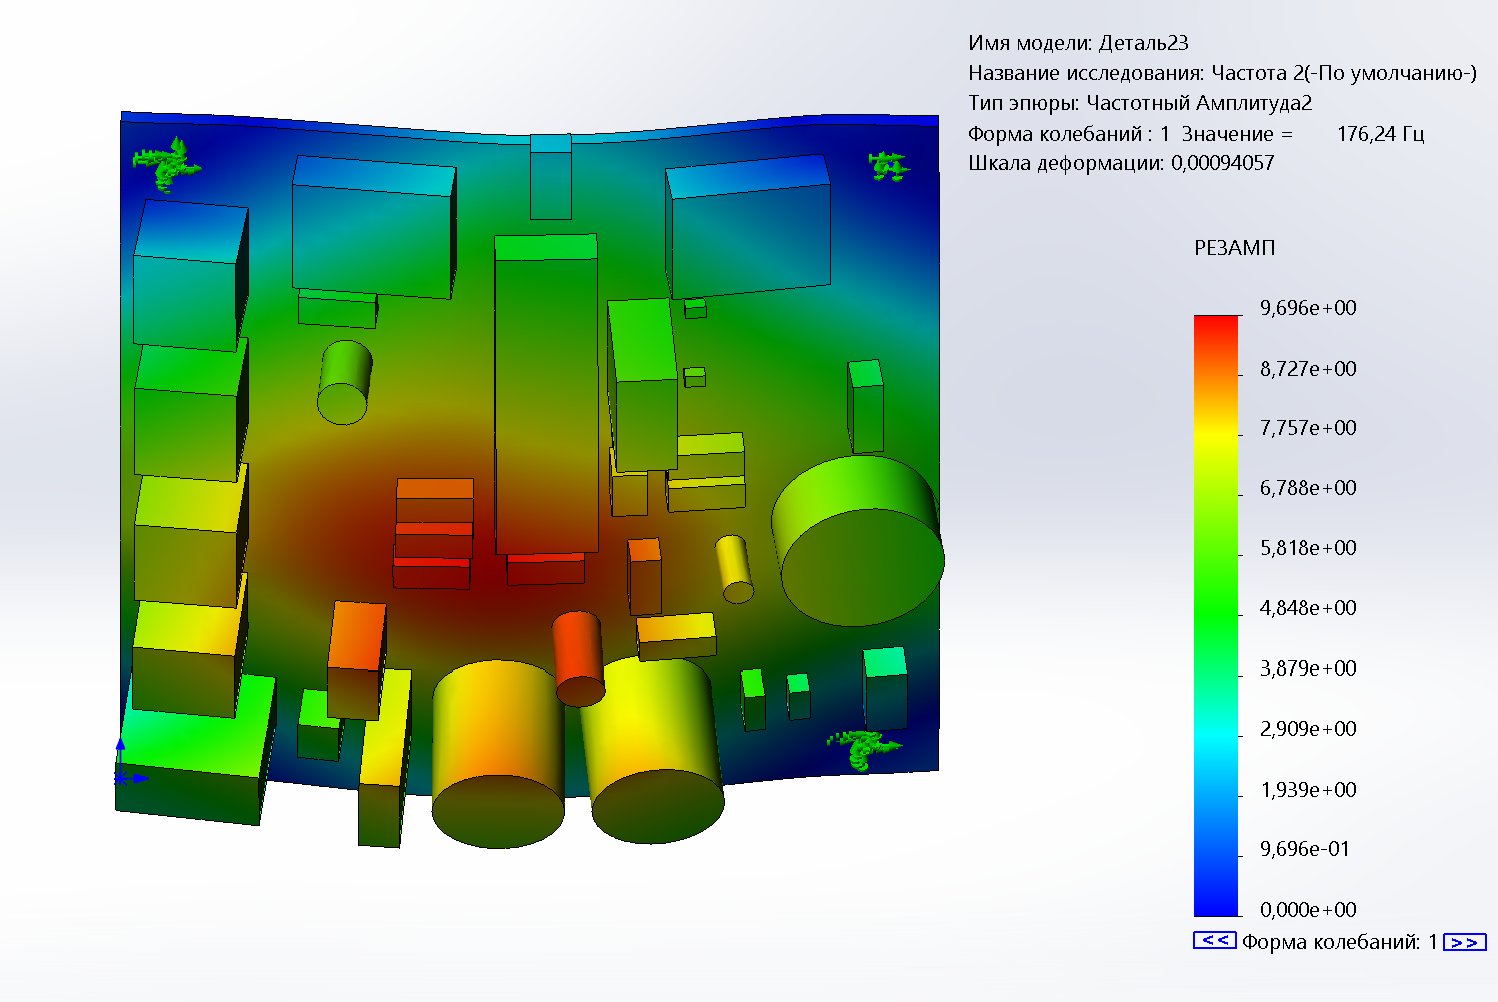
\includegraphics[scale=0.5]{solid.modeling/Amplitude-2-1.png}
  \caption{Результат эксперемента в SolidWorks Simulation (вариант 2)}
\end{figure}

\begin{figure}[H]
  \centering
  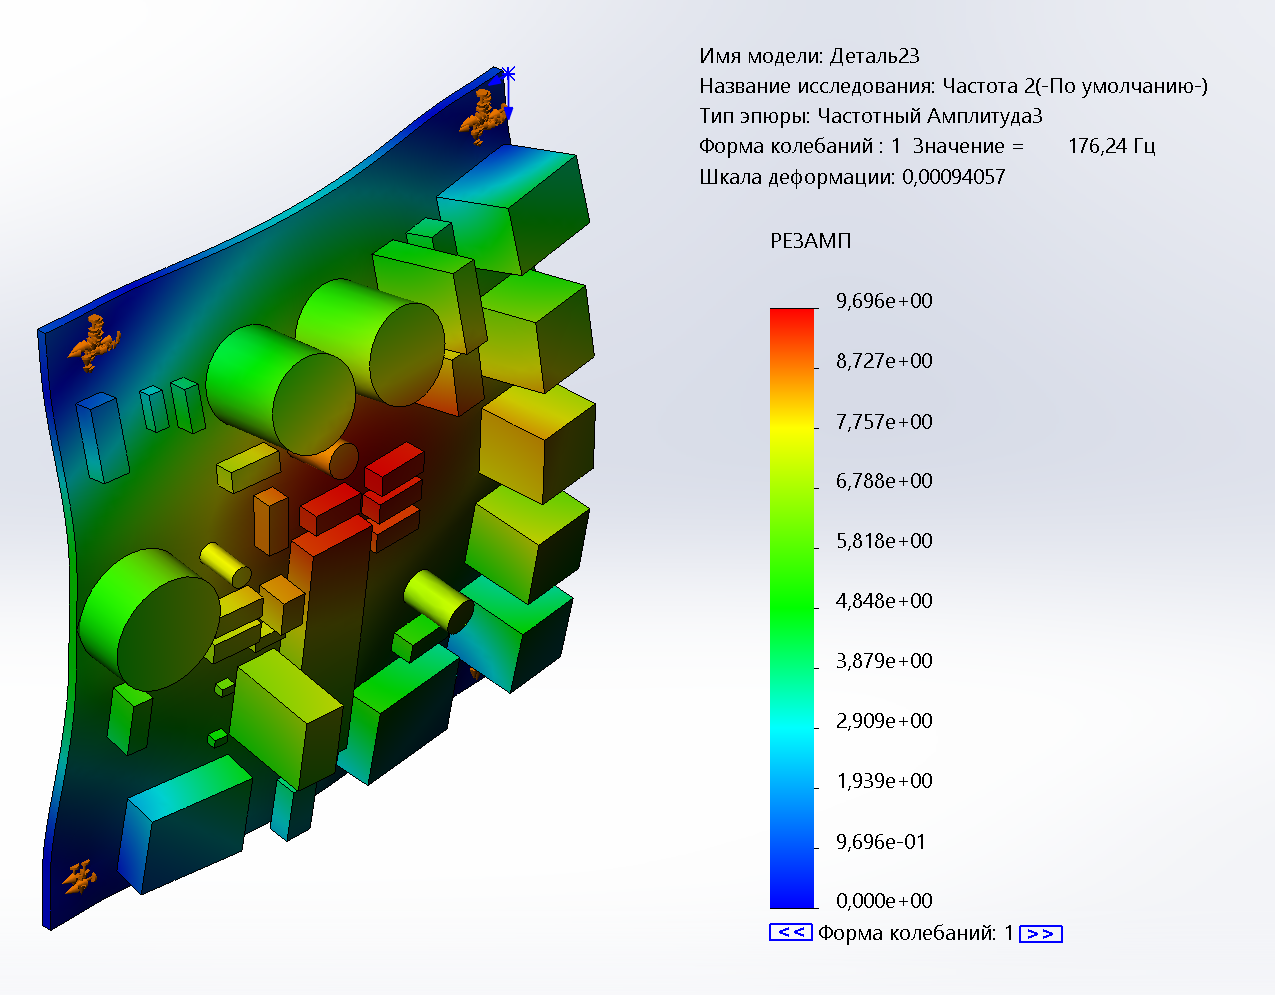
\includegraphics[scale=0.5]{solid.modeling/Amplitude-3-1.png}
  \caption{Результат эксперемента в SolidWorks Simulation (вариант 3)}
\end{figure}
\subsection{Технология моделирования тепловых процессов,
протекающих в электронном модуле и устройстве в целом с
использованием ANSYS, COMSOL Multiphysics, SolidWorks Simulation}


\subsection{Обработка, анализ и интерпретация данных результатов
моделирования программными средствами ANSYS, COMSOL Multiphysics,
SolidWorks Simulation.}




\newpage

%%% Local Variables:
%%% mode: LaTeX
%%% TeX-master: "main"
%%% End:
